
%{{第二十四回}}{第二十四回}}

\chapter{醉金刚轻财尚义侠\\痴女儿遗帕惹相思}\label{part0028_split_000.htmlux5cux23calibre_pb_0}

{}

{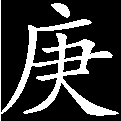
\includegraphics[width=3mm]{../Images/00004}夹写``醉金刚''一回是书中之大净场,聊醒看官倦眼耳。然亦书中必不可少之文,必不可少之人。今写在市井俗人身上,又加一``侠''字,则大有深意存焉。}

话说林黛玉正自情思萦逗,缠绵固结之时,忽有人从背后击了一掌,说道:``你作什么一个人在这里?''林黛玉倒唬了一跳,回头看时,不是别人,却是香菱。林黛玉道:``你这个傻{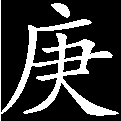
\includegraphics[width=3mm]{../Images/00004}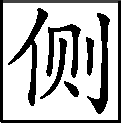
\includegraphics[width=3mm]{../Images/00011}\footnotesize \kaishu 此``傻''字加于香菱,则有多少丰神跳于纸上,其娇憨之态可想而知。}丫头,唬我这么一跳好的。你这会子打那里来?''香菱嘻嘻的笑道:``我来寻我们的姑娘的,找他总找不着。你们紫鹃也找你呢,{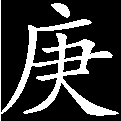
\includegraphics[width=3mm]{../Images/00004}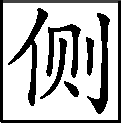
\includegraphics[width=3mm]{../Images/00011}\footnotesize \kaishu 一丝不漏。}说琏二奶奶送了什么茶叶来给你的。走罢,回家去坐着。''{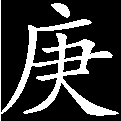
\includegraphics[width=3mm]{../Images/00004}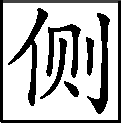
\includegraphics[width=3mm]{../Images/00011}\footnotesize \kaishu ``回家去坐着''之言,是恐石上冷意。}一面说着,一面拉着黛玉的手回潇湘馆来了。果然凤姐儿送了两小瓶上用新茶来。林黛玉和香菱坐了。况他们有甚正事谈讲。{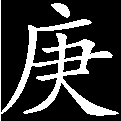
\includegraphics[width=3mm]{../Images/00004}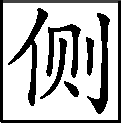
\includegraphics[width=3mm]{../Images/00011}\footnotesize \kaishu 为学诗伏线。}不过说些这一个绣的好,那一个刺的精,又下一回棋,看两句书,{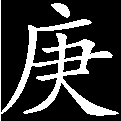
\includegraphics[width=3mm]{../Images/00004}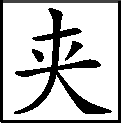
\includegraphics[width=3mm]{../Images/00012}\footnotesize \kaishu 棋不论盘,书不论章,皆是娇憨女儿神理,写得不即不离,似有似无,妙极!}香菱便走了。不在话下。{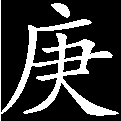
\includegraphics[width=3mm]{../Images/00004}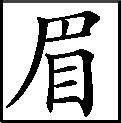
\includegraphics[width=3mm]{../Images/00010}\footnotesize \kaishu 是书最好看如此等处,系画家山水、树头、丘壑俱备,末用浓淡墨点苔法也。丁亥夏。畸笏叟。}

如今且说宝玉因被袭人找回房去,果见鸳鸯歪在床上看袭人的针线呢,见宝玉来了,便说道:``你往那里去了?老太太等着你呢,叫你过那边请大老爷的安去。还不快换了衣服走呢。''袭人便进房去取衣服。宝玉坐在床沿上,褪了鞋等靴子穿的工夫,回头见鸳鸯穿着水红绫子袄儿,青缎子背心,束着白绉绸汗巾儿,脸向那边低着头看针线,脖子上戴着花领子。宝玉便把脸凑在他脖项上,闻那粉香油气,不住用手摩挲,其白腻不在袭人之下,便猴上身去涎皮笑道:``好姐姐,把你嘴上的胭脂赏我吃了罢。''{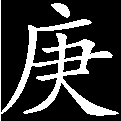
\includegraphics[width=3mm]{../Images/00004}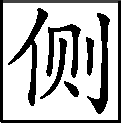
\includegraphics[width=3mm]{../Images/00011}\footnotesize \kaishu 胭脂是这样吃法。看官可经过否?}一面说着,一面扭股糖似的粘在身上。

鸳鸯便叫道:``袭人,你出来瞧瞧。{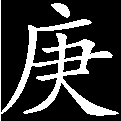
\includegraphics[width=3mm]{../Images/00004}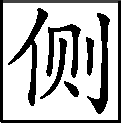
\includegraphics[width=3mm]{../Images/00011}\footnotesize \kaishu 不向宝玉说话,又叫袭人,鸳鸯亦是幻情洞天也。}你跟他一辈子,也不劝劝,还是这么着。''袭人抱了衣服出来,向宝玉道:``左劝也不改,右劝也不改,你到底是怎么样?你再这么着,{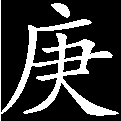
\includegraphics[width=3mm]{../Images/00004}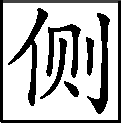
\includegraphics[width=3mm]{../Images/00011}\footnotesize \kaishu 此五字内有深意深心。}这个地方可就难住了。''一边说,一边催他穿了衣服,同鸳鸯往前面来见贾母。

见过贾母,出至外面,人马俱已齐备。刚欲上马,只见贾琏请安回来了,{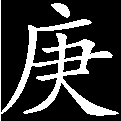
\includegraphics[width=3mm]{../Images/00004}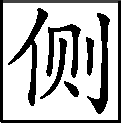
\includegraphics[width=3mm]{../Images/00011}\footnotesize \kaishu 一丝不漏。}正下马,二人对面,彼此问了两句话。只见旁边转出一个人来,{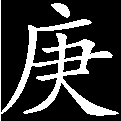
\includegraphics[width=3mm]{../Images/00004}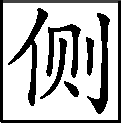
\includegraphics[width=3mm]{../Images/00011}\footnotesize \kaishu 芸哥此处一现,后文不见突然。}``请宝叔安''。宝玉看时,只见这人容长脸,长挑身材,年纪只好十八九岁,生得着实斯文清秀,倒也十分面善,只是想不起是那一房的,{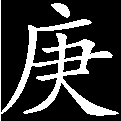
\includegraphics[width=3mm]{../Images/00004}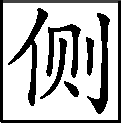
\includegraphics[width=3mm]{../Images/00011}\footnotesize \kaishu 大族人众,毕真,有是理。}叫什么名字。贾琏笑道:``你怎么发呆,连他也不认得?他是后廊上住的五嫂子的儿子芸儿。''宝玉笑道:``是了,是了,我怎么就忘了。''因问他母亲好,这会子什么勾当。贾芸指贾琏道:``找二叔说句话。''宝玉笑道:``你倒比先越发出挑了,{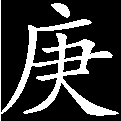
\includegraphics[width=3mm]{../Images/00004}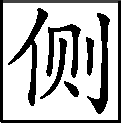
\includegraphics[width=3mm]{../Images/00011}\footnotesize \kaishu 何尝是十二三岁小孩语。}倒像我的儿子。''贾琏笑道:``好不害臊!人家比你大四五岁呢,就替你作儿子了?''宝玉笑道:``你今年十几岁了?''贾芸道:``十八岁。''

原来这贾芸最伶俐乖觉,听宝玉这样说,便笑道:``俗语说的,`摇车里的爷爷,拄拐的孙孙'。虽然岁数大,山高高不过太阳。只从我父亲没了,这几年也无人照管教导。{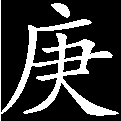
\includegraphics[width=3mm]{../Images/00004}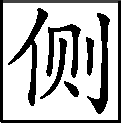
\includegraphics[width=3mm]{../Images/00011}\footnotesize \kaishu 虽是随机而应,伶俐人之语,余却伤心。}如若宝叔不嫌侄儿蠢笨,认作儿子,就是我的造化了。''贾琏笑道:``你听见了?认儿子不是好开交的呢。''{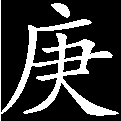
\includegraphics[width=3mm]{../Images/00004}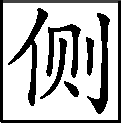
\includegraphics[width=3mm]{../Images/00011}\footnotesize \kaishu 是兄凑弟趣,可叹!}说着就进去了。宝玉笑道:``明儿你闲了,只管来找我,别和他们鬼鬼祟祟的。{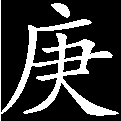
\includegraphics[width=3mm]{../Images/00004}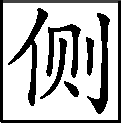
\includegraphics[width=3mm]{../Images/00011}\footnotesize \kaishu 何其堂皇正大之语。}这会子我不得闲儿。明儿你到书房里来,和你说天话儿,我带你园里顽耍去。''说着扳鞍上马,众小厮围随往贾赦这边来。

见了贾赦,不过是偶感些风寒,先述了贾母问的话,然后自己请了安。贾赦先站起来回了贾母话,{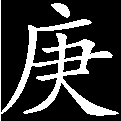
\includegraphics[width=3mm]{../Images/00004}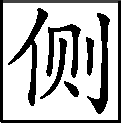
\includegraphics[width=3mm]{../Images/00011}\footnotesize \kaishu 一丝不乱。}次后便唤人来:``带哥儿进去太太屋里坐着。''宝玉退出,来至后面,进入上房。邢夫人见了他来,先倒站了起来请过贾母安,{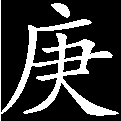
\includegraphics[width=3mm]{../Images/00004}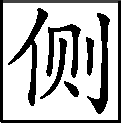
\includegraphics[width=3mm]{../Images/00011}\footnotesize \kaishu 一丝不乱。}宝玉方请安。{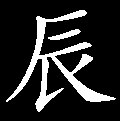
\includegraphics[width=3mm]{../Images/00009}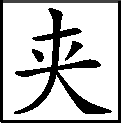
\includegraphics[width=3mm]{../Images/00012}\footnotesize \kaishu 好规矩。}邢夫人拉他上炕坐了,方问别人好,又命人倒茶来。{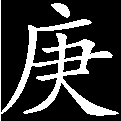
\includegraphics[width=3mm]{../Images/00004}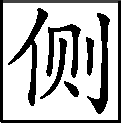
\includegraphics[width=3mm]{../Images/00011}\footnotesize \kaishu 好层次,好礼法,谁家故事?}一钟茶未吃完,只见那贾琮来问宝玉好。邢夫人道:``那里找活猴儿去!你那奶妈子死绝了,也不收拾收拾你,弄的黑眉乌嘴的,那里像大家子念书的孩子!''

正说着,只见贾环、贾兰小叔侄两个也来了,请过安,邢夫人便叫他两个椅子上坐了。贾环见宝玉同邢夫人坐在一个坐褥上,邢夫人又百般摩挲抚弄他,早已心中不自在了,{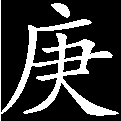
\includegraphics[width=3mm]{../Images/00004}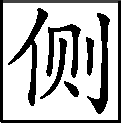
\includegraphics[width=3mm]{../Images/00011}\footnotesize \kaishu 千里伏线。}坐不多时,便和贾兰使眼色儿要走。贾兰只得依他,一同起身告辞。宝玉见他们要走,自己也就起身,要一同回去。邢夫人笑道:``你且坐着,我还和你说话呢。''宝玉只得坐了。邢夫人向他两个道:``你们回去,各人替我问你们各人母亲好。你们姑娘、姐姐妹妹都在这里呢,闹的我头晕,今儿不留你们吃饭了。''{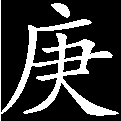
\includegraphics[width=3mm]{../Images/00004}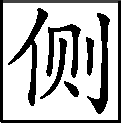
\includegraphics[width=3mm]{../Images/00011}\footnotesize \kaishu 明显薄情之至。}贾环等答应着,便出来回家去了。

宝玉笑道:``可是姐姐们都过来了,怎么不见?''邢夫人道:``他们坐了一会子,都往后头不知那屋里去了。''宝玉道:``大娘方才说有话说,不知是什么话?''邢夫人笑道:``那里有什么话,不过是叫你等着,同你姊妹们吃了饭去。还有一个好玩的东西给你带回去玩。''娘儿两个说话,不觉早又晚饭时节。调开桌椅,罗列杯盘,母女姊妹们吃毕了饭。宝玉去辞别了贾赦,同姊妹们一同回家,见过贾母、王夫人等,各自回房安息。不在话下。{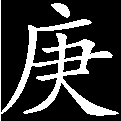
\includegraphics[width=3mm]{../Images/00004}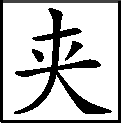
\includegraphics[width=3mm]{../Images/00012}\footnotesize \kaishu 一段为五鬼魇魔法作引。脂砚。}

且说贾芸进去见了贾琏,因打听可有什么事情。贾琏告诉他:``前儿倒有一件事情出来,偏生你婶子再三求了我,{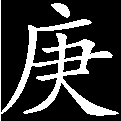
\includegraphics[width=3mm]{../Images/00004}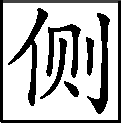
\includegraphics[width=3mm]{../Images/00011}\footnotesize \kaishu 反说体面话,惧内人累累如是。}给了贾芹了。他许了我,说明儿园里还有几处要栽花木的地方,等这个工程出来,一定给你就是了。''贾芸听了,半晌说道:``既是这样,我就等着罢。叔叔也不必先在婶子跟前提我今儿来打听的话,{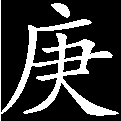
\includegraphics[width=3mm]{../Images/00004}\includegraphics[width=3mm]{../Images/00011}\footnotesize \kaishu 已得了主意了。}到跟前再说也不迟。''贾琏道:``提他作什么,{\includegraphics[width=3mm]{../Images/00004}\includegraphics[width=3mm]{../Images/00011}\footnotesize \kaishu 已被芸哥瞒过了。}我那里有这些工夫说闲话儿呢。明儿一个五更,还要到兴邑去走一趟,须得当日赶回来才好。你先去等着,后日起更以后你来讨信儿,来早了我不得闲。''说着便回后面换衣服去了。

贾芸出了荣国府回家,一路思量,想出一个主意来,便一径往他母舅卜世仁{\includegraphics[width=3mm]{../Images/00009}\includegraphics[width=3mm]{../Images/00012}\footnotesize \kaishu 名义可思。}家来。{\includegraphics[width=3mm]{../Images/00004}\includegraphics[width=3mm]{../Images/00011}\footnotesize \kaishu 既云``不是人'',如何肯共事?想芸哥此来空了。}原来卜世仁现开香料铺,方才从铺子里来,忽见贾芸进来,彼此见过了,因问他这早晚什么事跑了来。贾芸道:``有件事求舅舅帮衬帮衬。我有一件事,用些冰片麝香使用,好歹舅舅每样赊四两给我,八月里按数送了银子来。''{\includegraphics[width=3mm]{../Images/00004}\includegraphics[width=3mm]{../Images/00012}\footnotesize \kaishu 甥舅之谈如此,叹叹!}卜世仁冷笑道:``再休提赊欠一事。{\includegraphics[width=3mm]{../Images/00004}\includegraphics[width=3mm]{../Images/00011}\footnotesize \kaishu 何如,何如?余言不谬。}前儿也是我们铺子里一个伙计,替他的亲戚赊了几两银子的货,至今总未还上。因此我们大家赔上,立了合同,再不许替亲友赊欠。谁要赊欠,就要罚他二十两银子的东道。况且如今这个货也短,你就拿现银子到我们这不三不四的铺子里来买,{\includegraphics[width=3mm]{../Images/00004}\includegraphics[width=3mm]{../Images/00011}\footnotesize \kaishu 推脱之辞。}也还没有这些,只好倒扁儿去。这是一。二则你那里有正经事,不过赊了去又是胡闹。你只说舅舅见你一遭儿就派你一遭儿不是。你小人儿家很不知好歹,也到底立个主见,赚几个钱,弄得穿是穿吃是吃的,我看着也喜欢。''

贾芸笑道:``舅舅说的倒干净。我父亲没的时候,我年纪又小,不知事。后来听见我母亲说,都还亏舅舅们在我们家出主意,料理的丧事。难道舅舅就不知道的,还是有一亩地两间房子,如今在我手里花了不成?巧媳妇做不出没米的粥来,叫我怎么样呢?还亏是我呢,要是别个,死皮赖脸三日两头儿来缠着舅舅,要三升米二升豆子的,舅舅也就没有法呢。''{\includegraphics[width=3mm]{../Images/00004}\includegraphics[width=3mm]{../Images/00011}\footnotesize \kaishu 芸哥亦善谈,井井有理。◇余二人亦不曾有是气。}

卜世仁道:``我的儿,舅舅要有,还不是该的。我天天和你舅母说,只愁你没算计儿。你但凡立的起来,到你大房里,就是他们爷儿们见不着,便下个气,和他们的管家或者管事的人们嬉和嬉和,{\includegraphics[width=3mm]{../Images/00004}\includegraphics[width=3mm]{../Images/00011}\footnotesize \kaishu 可怜可叹,余竟为之一哭。}也弄个事儿管管。前日我出城去,撞见了你们三房里的老四,骑着大叫驴,带着五辆车,有四五十和尚道士,{\includegraphics[width=3mm]{../Images/00004}\includegraphics[width=3mm]{../Images/00012}\footnotesize \kaishu 妙极!写小人口角,羡慕之言加一倍,毕肖。却又是背面傅粉法。}往家庙去了。他那不亏能干,就有这样的事到他了!''贾芸听他韶刀的不堪,便起身告辞。{\includegraphics[width=3mm]{../Images/00004}\includegraphics[width=3mm]{../Images/00011}\footnotesize \kaishu 有志气,有果断。}卜世仁道:``怎么急的这样,吃了饭再去罢。''一句未完,只见他娘子说道:``你又糊涂了。{\includegraphics[width=3mm]{../Images/00004}\includegraphics[width=3mm]{../Images/00011}\footnotesize \kaishu 虽写小人家涩细,一吹一唱,酷肖之至,却是一气逼出,后文方不突然。《石头记》笔仗全在如此样者。}说着没有米,这里买了半斤面来下给你吃,这会子还装胖呢。留下外甥挨饿不成?''卜世仁说:``再买半斤来添上就是了。''他娘子便叫女孩儿:``银姐,往对门王奶奶家去问,有钱借二三十个,明儿就送过来。''夫妻两个说话,那贾芸早说了几个``不用费事'',去的无影无踪了。{{\includegraphics[width=3mm]{../Images/00004}\includegraphics[width=3mm]{../Images/00011}\footnotesize \kaishu 有知识有果断人,自是不同。} \includegraphics[width=3mm]{../Images/00009}\includegraphics[width=3mm]{../Images/00012}\footnotesize \kaishu 世情写透。}

不言卜家夫妇,且说贾芸赌气离了母舅家门,一径回归旧路,心下正自烦恼,一边想,一边低头只管走,不想一头就碰在一个醉汉身上,把贾芸唬了一跳。{\includegraphics[width=3mm]{../Images/00004}\includegraphics[width=3mm]{../Images/00011}\footnotesize \kaishu 自上看来,可是一口气否?}听那醉汉骂道:``臊你娘的!瞎了眼睛,碰起我来了。''贾芸忙要躲身,早被那醉汉一把抓住,对面一看,不是别人,却是紧邻倪二。原来这倪二是个泼皮,专放重利债,在赌博场吃闲钱,专管打降吃酒。如今正从欠钱人家索了利钱,吃醉回来,不想被贾芸碰了一头,正没好气,抡拳就要打。{\includegraphics[width=3mm]{../Images/00004}\includegraphics[width=3mm]{../Images/00010}\footnotesize \kaishu 这一节对《水浒记》杨志卖大刀遇没毛大虫一回看,觉好看多矣。己卯冬夜。脂砚。}只听那人叫道:``老二住手!是我冲撞了你。''倪二听见是熟人的语音,将醉眼睁开看时,见是贾芸,忙把手松了,趔趄着笑道:{\includegraphics[width=3mm]{../Images/00004}\includegraphics[width=3mm]{../Images/00011}\footnotesize \kaishu 写生之笔。}``原来是贾二爷,{\includegraphics[width=3mm]{../Images/00004}\includegraphics[width=3mm]{../Images/00011}\footnotesize \kaishu 如此称呼,可知芸哥素日行止,是``金盆虽破分两在''也。}我该死,我该死。这会子往那里去?''贾芸道:``告诉不得你,平白的又讨了个没趣儿。''{\includegraphics[width=3mm]{../Images/00004}\includegraphics[width=3mm]{../Images/00011}\footnotesize \kaishu 本无心之谈也。}倪二道:``不妨不妨,{\includegraphics[width=3mm]{../Images/00004}\includegraphics[width=3mm]{../Images/00011}\footnotesize \kaishu 如闻。}有什么不平的事,告诉我,替你出气。{\includegraphics[width=3mm]{../Images/00004}\includegraphics[width=3mm]{../Images/00011}\footnotesize \kaishu 写得酷肖,总是渐次逼出,不见一丝勉强。}这三街六巷,凭他是谁,有人得罪了我醉金刚倪二的街坊,管叫他人离家散!''贾芸道:``老二,你且别气,听我告诉你这原故。''{\includegraphics[width=3mm]{../Images/00004}\includegraphics[width=3mm]{../Images/00011}\footnotesize \kaishu 可是一顺而来?}说着,便把卜世仁一段事告诉了倪二。倪二听了大怒,``要不是令舅,我便骂不出好话来,{\includegraphics[width=3mm]{../Images/00004}\includegraphics[width=3mm]{../Images/00011}\footnotesize \kaishu 仗义人岂有不知礼者乎?何尝是破落户?冤杀金刚了。}真真气死我倪二。也罢,你也不用愁烦,我这里现有几两银子,你若用什么,只管拿去买办。但只一件,你我作了这些年的街坊,我在外头有名放账,你却从没有和我张过口。也不知你厌恶我是个泼皮,{\includegraphics[width=3mm]{../Images/00004}\includegraphics[width=3mm]{../Images/00011}\footnotesize \kaishu 知己知彼之话。}怕低了你的身分,也不知是你怕我难缠,利钱重?若说怕利钱重,这银子我是不要利钱的,也不用写文约,若说怕低了你的身分,{\includegraphics[width=3mm]{../Images/00004}\includegraphics[width=3mm]{../Images/00011}\footnotesize \kaishu 知己知彼之话。}我就不敢借给你了,各自走开。''一面说,一面果然从搭包里掏出一卷银子来。

贾芸心下自思:``素日倪二虽然是泼皮无赖,却因人而使,{\includegraphics[width=3mm]{../Images/00004}\includegraphics[width=3mm]{../Images/00011}\footnotesize \kaishu 四字是评,难得难得,非豪杰不可当。}颇颇的有义侠之名。若今日不领他这情,怕他臊了,倒恐生事。不如借了他的,改日加倍还他也倒罢了。''想毕笑道:``老二,你果然是个好汉,我何曾不想着你,和你张口。但只是我见你所相与交结的,都是些有胆量的有作为的人,似我们这等无能无为的你倒不理。{\includegraphics[width=3mm]{../Images/00004}\includegraphics[width=3mm]{../Images/00011}\footnotesize \kaishu 芸哥亦善谈,好口齿。}我若和你张口,你岂肯借给我。今日既蒙高情,我怎敢不领,回家按例写了文约过来便是了。''倪二大笑道:``好会说话的人。我却听不上这话。{\includegraphics[width=3mm]{../Images/00004}\includegraphics[width=3mm]{../Images/00011}\footnotesize \kaishu ``光棍眼内揉不下沙子''是也。}既说`相与交结'四个字,如何放账给他,使他的利钱!{\includegraphics[width=3mm]{../Images/00004}\includegraphics[width=3mm]{../Images/00011}\footnotesize \kaishu 如今不单是亲友言利,不但亲友,即闺阁中亦然,不但生意新发户,即大户旧族颇颇有之。}既把银子借与他,图他的利钱,便不是相与交结了。闲话也不必讲。既肯青目,这是十五两三钱有零的银子,便拿去治买东西。你要写什么文契,趁早把银子还我,让我放给那些有指望的人使去。''{\includegraphics[width=3mm]{../Images/00004}\includegraphics[width=3mm]{../Images/00011}\footnotesize \kaishu 爽快人,爽快话。}贾芸听了,一面接了银子,一面笑道:``我便不写罢了,有何着急的。''倪二笑道:``这不是话。天气黑了,也不让茶让酒,我还到那边有点事情去,你竟请回去。我还求你带个信儿与舍下,叫他们早些关门睡罢,我不回家去了,倘或有要紧事儿,叫我们女儿明儿一早到马贩子王短腿家{\includegraphics[width=3mm]{../Images/00004}\includegraphics[width=3mm]{../Images/00011}\footnotesize \kaishu 常起坐处人,毕真。}来找我。''一面说,一面趔趄着脚儿去了,{\includegraphics[width=3mm]{../Images/00004}\includegraphics[width=3mm]{../Images/00011}\footnotesize \kaishu 仍应前。}不在话下。{{\includegraphics[width=3mm]{../Images/00004}\includegraphics[width=3mm]{../Images/00010}\footnotesize \kaishu 读阅``醉金刚''一回,{(务)}{[}如{]}吃刘铉丹家山楂丸一付,一笑。◇余卅年来得遇金刚之样人不少,不及金刚者亦不少,惜书上不便历历注上芳讳,是余不{(是)}{[}足{]}心事也。壬午孟夏。}}

且说贾芸偶然碰了这件事,心中也十分罕希,想那倪二倒果然有些意思,只是还怕他一时醉中慷慨,到明日加倍的要起来,便怎处,心内犹豫不决。{\includegraphics[width=3mm]{../Images/00004}\includegraphics[width=3mm]{../Images/00011}\footnotesize \kaishu 芸哥实怕倪二,并非以小人之心度君子也。}忽又想道:``不妨,等那件事成了,也可加倍还他。''想毕,一直走到个钱铺里,将那银子称一称,十五两三钱四分二厘。贾芸见倪二不撒谎,心下越发欢喜,收了银子,来至家门,先到隔壁将倪二的信捎了与他娘子知道,方回家来。见他母亲自在炕上拈线,见他进来,便问那去了一日。贾芸恐他母亲生气,便不说起卜世仁的事来,{\includegraphics[width=3mm]{../Images/00004}\includegraphics[width=3mm]{../Images/00011}\footnotesize \kaishu 孝子可敬。此人后来荣府事败,必有一番作为。}只说在西府里等琏二叔的,问他母亲吃了饭不曾。他母亲已吃过了,说留的饭在那里。小丫头子拿过来与他吃。那天已是掌灯时候,贾芸吃了饭收拾歇息,一宿无话。

次日一早起来,洗了脸,便出南门,大香铺里买了冰麝,便往荣国府来。打听贾琏出了门,贾芸便往后面来。

到贾琏院门前,只见几个小厮拿着大高笤帚在那里扫院子呢。忽见周瑞家的从门里出来叫小厮们:``先别扫,奶奶出来了。''贾芸忙上前笑问:``二婶婶那去?''周瑞家的道:``老太太叫,想必是裁什么尺头。''正说着,只见一群人簇着凤姐出来了。{\includegraphics[width=3mm]{../Images/00004}\includegraphics[width=3mm]{../Images/00011}\footnotesize \kaishu 当家人有是派头。}贾芸深知凤姐是喜奉承尚排场的,{\includegraphics[width=3mm]{../Images/00004}\includegraphics[width=3mm]{../Images/00011}\footnotesize \kaishu 那一个不喜奉承。}忙把手逼着,恭恭敬敬抢上来请安。凤姐连正眼也不看,仍往前走着,只问他母亲好,``怎么不来我们这里逛逛?''贾芸道:``只是身上不大好,倒时常记挂着婶子,要来瞧瞧,又不能来。''凤姐笑道:``可是会撒谎,不是我提起他来,你就不说他想我了。''贾芸笑道:``侄儿不怕雷打了,就敢在长辈前撒谎。昨儿晚上还提起婶子来,说婶子身子生的单弱,事情又多,亏婶子好大精神,竟料理的周周全全,要是差一点儿的,早累的不知怎么样呢。''{\includegraphics[width=3mm]{../Images/00004}\includegraphics[width=3mm]{../Images/00010}\footnotesize \kaishu 自往卜世仁处去已安排下的。芸哥可用。己卯冬夜。}

凤姐听了满脸是笑,不由的便止了步,问道:``怎么好好的你娘儿们在背地里嚼起我来?''{\includegraphics[width=3mm]{../Images/00004}\includegraphics[width=3mm]{../Images/00011}\footnotesize \kaishu 过下无痕,天然而来文字。}贾芸道:``有个原故,{\includegraphics[width=3mm]{../Images/00004}\includegraphics[width=3mm]{../Images/00011}\footnotesize \kaishu 接得如何?}只因我有个朋友,家里有几个钱,现开香铺。只因他身上捐着个通判,前儿选了云南不知那一处,{\includegraphics[width=3mm]{../Images/00004}\includegraphics[width=3mm]{../Images/00011}\footnotesize \kaishu 随口语,极妙!}连家眷一齐去,把这香铺也不在这里开了。便把账物攒了一攒,该给人的给人,该贱发的贱发了,{\includegraphics[width=3mm]{../Images/00006}\includegraphics[width=3mm]{../Images/00011}\footnotesize \kaishu 世法人情,随便招来,皆是奇妙文章。}像这细贵的货,都分着送与亲朋。他就一共送了我些冰片、麝香。我就和我母亲商量,{\includegraphics[width=3mm]{../Images/00004}\includegraphics[width=3mm]{../Images/00011}\footnotesize \kaishu 像得紧,何尝撒谎?}若要转卖,不但卖不出原价来,而且谁家拿这些银子买这个作什么,便是很有钱的大家子,也不过使个几分几钱就挺折腰了,若说送人,也没个人配使这些,{\includegraphics[width=3mm]{../Images/00006}\includegraphics[width=3mm]{../Images/00011}\footnotesize \kaishu 作者是何神圣,具此等大光明眼,无微不照?}倒叫他一文不值半文转卖了。因此我就想起婶子来。{\includegraphics[width=3mm]{../Images/00006}\includegraphics[width=3mm]{../Images/00011}\footnotesize \kaishu 为大千世界一哭。}往年间我还见婶子大包的银子买这些东西呢,别说今年贵妃宫中,就是这个端阳节下,不用说这些香料自然是比往常加上十倍去的。因此想来想去,只孝顺婶子一个人才合式,{\includegraphics[width=3mm]{../Images/00006}\includegraphics[width=3mm]{../Images/00011}\footnotesize \kaishu 有此一番必当孝顺、必当收下、必得备用之情景,行文{(妙)}{[}好{]}看杀人,立意{(稀)}{[}奚{]}落杀人,看至此不知当哭当笑。}方不算遭塌这东西。''一边说,一边将一个锦匣举起来。

凤姐正是要办端阳的节礼,采买香料药饵的时节,忽见贾芸如此一来,听这一篇话,心下又是得意又是欢喜,{\includegraphics[width=3mm]{../Images/00006}\includegraphics[width=3mm]{../Images/00011}\footnotesize \kaishu 逼真。}便命丰儿:``接过芸哥儿的来,{\includegraphics[width=3mm]{../Images/00004}\includegraphics[width=3mm]{../Images/00011}\footnotesize \kaishu 像个婶子口气,好看煞!}送了家去,交给平儿。''因又说道:``看着你这样知好歹,怪道你叔叔常提你,说你说话儿也明白,心里有见识。''{\includegraphics[width=3mm]{../Images/00004}\includegraphics[width=3mm]{../Images/00012}\footnotesize \kaishu 看官须记,凤姐所喜者,是奉承之言,打动了心,不是见物而欢喜,若说是见物而喜,便不是阿凤矣。}贾芸听这话入了港,便打进一步来,故意问道:``原来叔叔也曾提我的?''凤姐见问,才要告诉他与他管事情的那话,便忙又止住,心下想道:{\includegraphics[width=3mm]{../Images/00004}\includegraphics[width=3mm]{../Images/00011}\footnotesize \kaishu 的是阿凤行事心机笔意。}``我如今要告诉他那话,倒叫他看着我见不得东西似的,为得了这点子香,就混许他管事了。今儿先别提起这事。''想毕,便把派他监种花木工程的事都隐瞒的一字不提,随口说了两句淡话,便往贾母那里去了。贾芸也不好提的,只得回来。

因昨日见了宝玉,叫他到外书房等着,{\includegraphics[width=3mm]{../Images/00006}\includegraphics[width=3mm]{../Images/00011}\footnotesize \kaishu 一样叔婶,两般侍奉。}贾芸吃了饭便又进来,到贾母那边仪门外绮霰斋书房里来。只见茗烟\href{../Text/part0028_split_000.html\#lnkback_1_a}{\textsuperscript{①}}、锄药两个小厮下象棋,为夺``车''正拌嘴,还有引泉、扫花、挑云、伴鹤{\includegraphics[width=3mm]{../Images/00004}\includegraphics[width=3mm]{../Images/00011}\footnotesize \kaishu 好名色。}四五个,又在房檐上掏小雀儿玩。{\includegraphics[width=3mm]{../Images/00006}\includegraphics[width=3mm]{../Images/00011}\footnotesize \kaishu 行云流{[}水{]},一字不空。真是空灵活跳。}

贾芸进入院内,把脚一跺,说道:``猴头们淘气,我来了。''众小厮看见贾芸进来,都才散了。贾芸进入房内,便坐在椅子上问:``宝二爷没下来?''茗烟道:``今儿总没下来。二爷说什么,我替你哨探哨探去。''{\includegraphics[width=3mm]{../Images/00004}\includegraphics[width=3mm]{../Images/00011}\footnotesize \kaishu 五遁之外,名曰``哨探遁''法。}说着,便出去了。这里贾芸便看字画古玩,有一顿饭工夫还不见来,再看看别的小厮,都顽去了。正是烦闷,只听门前娇声嫩语的叫了一声``哥哥''。

贾芸往外瞧时,看是一个十六七岁的丫头,生的倒也细巧干净。那丫头见了贾芸,便抽身躲了过去。{\includegraphics[width=3mm]{../Images/00006}\includegraphics[width=3mm]{../Images/00011}\footnotesize \kaishu 是必然之理。}恰值茗烟走来,见那丫头在门前,便说道:``好,好,{\includegraphics[width=3mm]{../Images/00004}\includegraphics[width=3mm]{../Images/00011}\footnotesize \kaishu 二``好''字是遮饰半句来不到语。}正抓不着个信儿。''贾芸见了茗烟,也就赶了出来,问怎么样。茗烟道:``等了这一日,也没个人儿过来。这就是宝二爷房里的。好姑娘,{\includegraphics[width=3mm]{../Images/00004}\includegraphics[width=3mm]{../Images/00011}\footnotesize \kaishu 口气极像。}你进去带个信儿,就说廊上的二爷来了。''那丫头听说,方知是本家的爷们,便不似先前那等回避,{\includegraphics[width=3mm]{../Images/00004}\includegraphics[width=3mm]{../Images/00011}\footnotesize \kaishu 一句,礼当。}下死眼把贾芸钉了两眼。{{\includegraphics[width=3mm]{../Images/00004}\includegraphics[width=3mm]{../Images/00011}\footnotesize \kaishu 这句是情孽上生。 }\includegraphics[width=3mm]{../Images/00006}\includegraphics[width=3mm]{../Images/00011}\footnotesize \kaishu 五百年风流孽冤。}听那贾芸说道:``什么是廊上廊下的,你只说是芸儿就是了。''半晌,那丫头冷笑了一笑:{\includegraphics[width=3mm]{../Images/00004}\includegraphics[width=3mm]{../Images/00011}\footnotesize \kaishu 神情是深知房中事的。}``依我说,二爷竟请回家去,有什么话明儿再来。今儿晚上得空儿我回了他。''茗烟道:``这是怎么说?''那丫头道:``他{\includegraphics[width=3mm]{../Images/00004}\includegraphics[width=3mm]{../Images/00011}\footnotesize \kaishu 一连两个``他''字,怡红院中使得,否则有假矣。}今儿也没睡中觉,自然吃的晚饭早。晚上他又不下来。难道只是耍的二爷在这里等着挨饿不成!{\includegraphics[width=3mm]{../Images/00006}\includegraphics[width=3mm]{../Images/00011}\footnotesize \kaishu 业已种下爱根,俟后无计可拔。}不如家去,明儿来是正经。便是回来有人带信,那都是不中用的。他不过口里应着,他倒给带呢!''贾芸听这丫头说话简便俏丽,待要问他的名字,因是宝玉房里的,又不便问,只得说道:``这话倒是,我明儿再来。''说着便往外走。茗烟道:``我倒茶去,{\includegraphics[width=3mm]{../Images/00004}\includegraphics[width=3mm]{../Images/00011}\footnotesize \kaishu 滑贼。}二爷吃了茶再去。''贾芸一面走,一面回头说:``不吃茶,我还有事呢。''口里说话,眼睛瞧那丫头还站在那里呢。

那贾芸一径回家。至次日来至大门前,可巧遇见凤姐往那边去请安,才上了车,见贾芸来,便命人唤住,隔窗子笑道:``芸儿,你竟有胆子在我的跟前弄鬼。{\includegraphics[width=3mm]{../Images/00004}\includegraphics[width=3mm]{../Images/00011}\footnotesize \kaishu 也作的不像撒谎,用心机人可怕是此等处。}怪道你送东西给我,原来你有事求我。昨儿你叔叔才告诉我说你求他。''{\includegraphics[width=3mm]{../Images/00006}\includegraphics[width=3mm]{../Images/00011}\footnotesize \kaishu 非此等话法,则是因昨日之物起见了。锦心绣口,真真拜服。}贾芸笑道:``求叔叔这事,婶子休提,我昨儿正后悔呢。早知这样,我竟一起头求婶子,这会子也早完了。谁承望叔叔竟不能的。''{\includegraphics[width=3mm]{../Images/00006}\includegraphics[width=3mm]{../Images/00011}\footnotesize \kaishu 这样话实是以非理加之,而世人大都乐受喜闻,吾深怪之。}凤姐笑道:``怪道你那里没成儿,昨儿又来寻我。''贾芸道:``婶子辜负了我的孝心,我并没有这个意思。若有这个意思,昨儿还不求婶子?如今婶子既知道了,我倒要把叔叔丢下,少不得求婶子好歹疼我一点儿。''凤姐冷笑道:``你们要拣远路儿走,叫我也难说。{\includegraphics[width=3mm]{../Images/00004}\includegraphics[width=3mm]{../Images/00011}\footnotesize \kaishu 曹操语。}早告诉我一声儿,有什么不成的,多大点子事,耽误到这会子。那园子里还要种花,我只想不出一个人来,你早来不早完了。''贾芸笑道:``既这样,婶子明儿就派我罢。''凤姐半晌道:``这个我看着不大好。{\includegraphics[width=3mm]{../Images/00004}\includegraphics[width=3mm]{../Images/00011}\footnotesize \kaishu 又一折。}等明年正月里烟火灯烛那个大宗儿下来,再派你罢。''贾芸道:``好婶子,先把这个派了我罢。果然这个办的好,再派我那个。''凤姐笑道:``你倒会拉长线儿。罢了,要不是你叔叔说,我不管你的事。{\includegraphics[width=3mm]{../Images/00004}\includegraphics[width=3mm]{../Images/00011}\footnotesize \kaishu 总不认受冰麝贿。}我也不过吃了饭就过来,你到午错的时候来领银子,后儿就进去种树。''说毕,令人驾起香车,一径去了。

贾芸喜不自禁,来至绮霰斋打听宝玉,谁知宝玉一早便往北静王府里去了。贾芸便呆呆的坐到晌午,打听凤姐回来,便写个领票来领对牌。至院外,命人通报了,彩明走了出来,单要了领票进去,批了银数年月,一并连对牌交与了贾芸。贾芸接了,看那批上银数批了二百两,心中喜不自禁,翻身走到银库上,交与收牌票的,领了银子。回家告诉母亲,自是母子俱各欢喜。次日一个五鼓,贾芸先找了倪二,将前银按数还他。那倪二见贾芸有了银子,他便按数收回,不在话下。这里贾芸又拿了五十两,出西门找到花儿匠方椿家里去买树,不在话下。{\includegraphics[width=3mm]{../Images/00004}\includegraphics[width=3mm]{../Images/00012}\footnotesize \kaishu 至此便完种树工程。◇一者见得趱赶工程原非正文,不过虚描盛时光景,借此以出情文。二者又为避难法。若不如此了,必曰其树其价、怎么买、定几株,岂不烦絮矣?}

如今且说宝玉,自那日见了贾芸,曾说明日着他进来说话儿。如此说了之后,他原是富贵公子的口角,那里还把这个放在心上,因而便忘怀了。{\includegraphics[width=3mm]{../Images/00004}\includegraphics[width=3mm]{../Images/00011}\footnotesize \kaishu 若是一个女孩儿,可保不忘的。}这日晚上,从北静王府里回来,见过贾母,王夫人等,回至园内,换了衣服,正要洗澡。袭人因被薛宝钗烦了去打结子,秋纹、碧痕两个去催水,檀云又因他母亲的生日接了出去,麝月又现在家中养病,虽还有几个作粗活听唤的丫头,估着叫不着他们,都出去寻伙觅伴的玩去了。不想这一刻的工夫,{\includegraphics[width=3mm]{../Images/00004}\includegraphics[width=3mm]{../Images/00012}\footnotesize \kaishu 妙!必用``一刻''二字方是宝玉的房中,见得时时原有人的,又有今一刻无人,所谓凑巧其一也。}只剩了宝玉在房内。偏生的{\includegraphics[width=3mm]{../Images/00004}\includegraphics[width=3mm]{../Images/00012}\footnotesize \kaishu 三字不可少。}宝玉要吃茶,一连叫了两三声,方见两三个老嬷嬷走进来。{\includegraphics[width=3mm]{../Images/00004}\includegraphics[width=3mm]{../Images/00012}\footnotesize \kaishu 妙!文字细密,一丝不落,非批得出者。}宝玉见了他们,连忙摇手儿说:``罢,罢,不用你们了。''{\includegraphics[width=3mm]{../Images/00004}\includegraphics[width=3mm]{../Images/00012}\footnotesize \kaishu 是宝玉口气。}老婆子们只得退出。

宝玉见没丫头们,只得自己下来,拿了碗向茶壶去倒茶。只听背后说道:``二爷仔细烫了手,让我们来倒。''{\includegraphics[width=3mm]{../Images/00004}\includegraphics[width=3mm]{../Images/00011}\footnotesize \kaishu 神龙变化之文,人岂能测?}一面说,一面走上来,早接了碗过去。宝玉倒唬了一跳,问:``你在那里的?忽然来了,唬我一跳。''那丫头一面递茶,一面回说:``我在后院子里,才从里间的后门进来,难道二爷就没听见脚步响?''宝玉一面吃茶,一面{\includegraphics[width=3mm]{../Images/00004}\includegraphics[width=3mm]{../Images/00012}\footnotesize \kaishu 六个``一面'',是神情,并不觉厌。}仔细打量那丫头:穿着几件半新不旧的衣裳,倒是一头黑鬒鬒的头发,挽着个?,容长脸面,细巧身材,却十分俏丽干净。{\includegraphics[width=3mm]{../Images/00004}\includegraphics[width=3mm]{../Images/00012}\footnotesize \kaishu 与贾芸目中所见不差。}宝玉看了,便笑问道:{\includegraphics[width=3mm]{../Images/00004}\includegraphics[width=3mm]{../Images/00012}\footnotesize \kaishu 神情写得出。}``你也是我这屋里的人么?''{\includegraphics[width=3mm]{../Images/00004}\includegraphics[width=3mm]{../Images/00012}\footnotesize \kaishu 妙问。必如此问方是笼络前文。}那丫头道:``是的。''宝玉道:``既是这屋里的,我怎么不认得?''那丫头听说,便冷笑了一声道:{\includegraphics[width=3mm]{../Images/00004}\includegraphics[width=3mm]{../Images/00012}\footnotesize \kaishu 神理如画。}``认不得的也多,岂只我一个。从来我又不递茶递水,拿东拿西,眼见的事一点儿不作,那里认得呢。''宝玉道:``你为什么不作那眼见的事?''{\includegraphics[width=3mm]{../Images/00004}\includegraphics[width=3mm]{../Images/00011}\footnotesize \kaishu 这是下情不能上达意语也。}那丫头道:``这话我也难说。{\includegraphics[width=3mm]{../Images/00004}\includegraphics[width=3mm]{../Images/00011}\footnotesize \kaishu 不伏气语,况非尔可完,故云``难说''。}只是有一句话回二爷:昨儿有个什么芸儿来找二爷。我想二爷不得空儿,便叫茗烟回他,叫他今日早起来,不想二爷又往北府里去了。''刚说到这句话,只见秋纹、碧痕嘻嘻哈哈的说笑着进来,两个人共提着一桶水,一手撩着衣裳,趔趔趄趄、泼泼撒撒的。那丫头便忙迎去接。{\includegraphics[width=3mm]{../Images/00004}\includegraphics[width=3mm]{../Images/00011}\footnotesize \kaishu 好!有眼色。}那秋纹、碧痕正对着抱怨,``你湿了我的裙子'',那个又说``你踹了我的鞋''。忽见走出一个人来接水,二人看时,不是别人,原来是小红。二人便都诧异,将水放下,忙进房来东瞧西望,{\includegraphics[width=3mm]{../Images/00004}\includegraphics[width=3mm]{../Images/00011}\footnotesize \kaishu 四字渐露大丫头素日怡红细事也。 \includegraphics[width=3mm]{../Images/00004}\includegraphics[width=3mm]{../Images/00010}\footnotesize \kaishu 怡红细事俱用带笔白描,是大章法也。丁亥夏。畸笏叟。}并没个别人,只有宝玉,便心中大不自在。只得预备下洗澡之物,待宝玉脱了衣裳,二人便带上门出来,{\includegraphics[width=3mm]{../Images/00004}\includegraphics[width=3mm]{../Images/00011}\footnotesize \kaishu 清楚之至。}走到那边房内便找小红,问他方才在屋里说什么。小红道:``我何曾在屋里的?只因我的手帕子不见了,往后头找手帕子去。不想二爷要茶吃,叫姐姐们一个没有,是我进去了,才倒了茶,姐姐们便来了。''秋纹听了,兜脸啐了一口,骂道:``没脸的下流东西!正经叫你去催水去,你说有事故,倒叫我们去,你可等着做这个巧宗儿。{\includegraphics[width=3mm]{../Images/00004}\includegraphics[width=3mm]{../Images/00011}\footnotesize \kaishu 难说小红无心,白描。}一里一里的,这不上来了。难道我们倒跟不上你了?你也拿镜子照照,配递茶递水不配!''{\includegraphics[width=3mm]{../Images/00004}\includegraphics[width=3mm]{../Images/00011}\footnotesize \kaishu ``难说''二字全在此句来。}碧痕道:``明儿我说给他们,凡要茶要水送东送西的事,咱们都别动,只叫他去便是了。''秋纹道:``这么说,不如我们散了,单让他在这屋里呢。''二人你一句我一句,正闹着,只见有个老嬷嬷进来传凤姐的话说:``明日有人带花儿匠来种树,叫你们严禁些,衣服裙子别混晒混晾的。那土山上一溜都拦着帏幕呢,可别混跑。''秋纹便问:{\includegraphics[width=3mm]{../Images/00004}\includegraphics[width=3mm]{../Images/00011}\footnotesize \kaishu 用秋纹问,是暗透之法。}``明儿不知是谁带进匠人来监工?''那婆子道:``说什么后廊上的芸哥儿。''秋纹、碧痕听了都不知道,只管混问别的话。那小红听见了,{\includegraphics[width=3mm]{../Images/00004}\includegraphics[width=3mm]{../Images/00011}\footnotesize \kaishu 可是暗透法?}心内却明白,就知是昨儿外书房所见那人了。

原来这小红本姓林,{\includegraphics[width=3mm]{../Images/00004}\includegraphics[width=3mm]{../Images/00012}\footnotesize \kaishu 又是个林。}小名红玉,{\includegraphics[width=3mm]{../Images/00004}\includegraphics[width=3mm]{../Images/00012}\footnotesize \kaishu ``红''字切``绛珠'',``玉''字则直通矣。}只因``玉''字犯了林黛玉、宝玉,{\includegraphics[width=3mm]{../Images/00004}\includegraphics[width=3mm]{../Images/00012}\footnotesize \kaishu 妙文。}便都把这个字隐起来,便都叫他``小红''。原是荣国府中世代的旧仆,他父母现在收管各处房田事务。这红玉年方十六岁,因分人在大观园的时节,把他便分在怡红院中,倒也清幽雅静。不想后来命人进来居住,偏生这一所儿又被宝玉占了。这红玉虽然是个不谙事的丫头,却因他有三分容貌,{\includegraphics[width=3mm]{../Images/00004}\includegraphics[width=3mm]{../Images/00012}\footnotesize \kaishu 有三分容貌尚且不肯受屈,况黛玉等一干才貌者乎?}心内着实妄想痴心的往上攀高,{\includegraphics[width=3mm]{../Images/00004}\includegraphics[width=3mm]{../Images/00012}\footnotesize \kaishu 争夺者同来一看。}每每的要在宝玉面前现弄现弄。只是宝玉身边一干人,都是伶牙利爪的,{\includegraphics[width=3mm]{../Images/00004}\includegraphics[width=3mm]{../Images/00011}\footnotesize \kaishu ``难说''的原故在此。}那里插的下手去。不想今儿才有些消息,{\includegraphics[width=3mm]{../Images/00004}\includegraphics[width=3mm]{../Images/00011}\footnotesize \kaishu 余前批不谬。}又遭秋纹等一场恶意,心内早灰了一半。{\includegraphics[width=3mm]{../Images/00004}\includegraphics[width=3mm]{../Images/00012}\footnotesize \kaishu 争名夺利者齐来一哭。}正闷闷的,忽然听见老嬷嬷说起贾芸来,不觉心中一动,便闷闷的回至房中,睡在床上暗暗盘算,翻来掉去,正没个抓寻。忽听窗外低低的叫道:``红玉,你的手帕子我拾在这里呢。''红玉听了忙走出来看,不是别人,正是贾芸。红玉不觉的粉面含羞,问道:``二爷在那里拾着的?''贾芸笑道:``你过来,我告诉你。''一面说,一面就上来拉他。那红玉急回身一跑,却被门槛绊倒。{\includegraphics[width=3mm]{../Images/00004}\includegraphics[width=3mm]{../Images/00011}\footnotesize \kaishu 睡梦中当然一跑,这方是怡红之鬟。}要知端的,下回分解。

{{\includegraphics[width=3mm]{../Images/00004}《红楼梦》写梦章法总不雷同。此梦更写的新奇,不见后文,不知是梦。}}

{{红玉在怡红院为诸鬟所掩,亦可谓生不遇时,但看后四章供阿凤驱使可知。}}

{\includegraphics[width=3mm]{../Images/00005}总评:冷暖时,只自知,金刚、卜氏浑闲事。眼中心,言中意,三生旧债原无底。任你贵比王侯,任你富似郭、石,一时间,风流愿,不怕死!}

{\href{../Text/part0028_split_000.html\#navto_1_a}{①}原作``焙茗''。宝玉的小厮``茗烟'',从本回至第三十四回称作``焙茗'',第三十九回以后又作``茗烟''。现统一为``茗烟''。}
